\documentclass[12pt,a4paper]{article}
\usepackage[utf8]{inputenc}
\usepackage[T1]{fontenc}
\usepackage{amsmath,amsfonts,amssymb}
\usepackage{graphicx}
\usepackage{xcolor}
\usepackage{listings}
\usepackage{hyperref}
\usepackage{geometry}
\usepackage{fancyhdr}
\usepackage{titlesec}
\usepackage{tocloft}
\usepackage{booktabs}
\usepackage{longtable}
\usepackage{float}

% Page setup
\geometry{
    left=2.5cm,
    right=2.5cm,
    top=2.5cm,
    bottom=2.5cm
}

% Fix header height
\setlength{\headheight}{14.5pt}

% Colors
\definecolor{kyosblue}{RGB}{30, 144, 255}
\definecolor{kyosdark}{RGB}{25, 25, 25}
\definecolor{kyosgreen}{RGB}{0, 255, 127}
\definecolor{kyosred}{RGB}{255, 69, 0}

% Code listings setup
\lstset{
    language=bash,
    basicstyle=\footnotesize\ttfamily,
    backgroundcolor=\color{gray!10},
    frame=single,
    rulecolor=\color{kyosblue},
    keywordstyle=\color{kyosblue}\bfseries,
    commentstyle=\color{gray}\itshape,
    stringstyle=\color{kyosred},
    numberstyle=\tiny\color{gray},
    breaklines=true,
    showstringspaces=false,
    tabsize=4,
    captionpos=b
}

% Header and footer
\pagestyle{fancy}
\fancyhf{}
\fancyhead[L]{\textcolor{kyosblue}{KyOS: The Dragon Arch - Technical Whitepaper}}
\fancyhead[R]{\textcolor{kyosblue}{\today}}
\fancyfoot[C]{\textcolor{kyosblue}{\thepage}}

% Title formatting
\titleformat{\section}{\Large\bfseries\color{kyosblue}}{\thesection}{1em}{}
\titleformat{\subsection}{\large\bfseries\color{kyosdark}}{\thesubsection}{1em}{}
\titleformat{\subsubsection}{\normalsize\bfseries\color{kyosdark}}{\thesubsubsection}{1em}{}

% Hyperlink setup
\hypersetup{
    colorlinks=true,
    linkcolor=kyosblue,
    filecolor=kyosblue,
    urlcolor=kyosblue,
    citecolor=kyosblue
}

\title{
    \Huge\textbf{\textcolor{kyosblue}{KyOS}}\\
    \Large\textcolor{kyosdark}{The Dragon Arch}\\
    \LARGE\textcolor{kyosdark}{Technical Whitepaper}\\
    \large\textcolor{gray}{A Modern, Security-Focused Arch Linux Distribution}\\
    \vspace{1cm}
    
\includegraphics[width=0.3\textwidth]{kyos.png}
}

\author{
    \textbf{Rahul Rajith}\\
    \texttt{rahulridhu21@gmail.com}\\
    \vspace{0.5cm}
    \textbf{Role:} Developer \& Architect\\
    \textbf{Project:} KyOS: The Dragon Arch\\
    \textbf{Version:} 2025.07\\
    \textbf{Classification:} Technical Documentation\\
    \vspace{0.5cm}
    \textbf{Website:} \url{https://ky-os.github.io/}\\
}

\date{\today}

\begin{document}

\maketitle
\thispagestyle{empty}

\newpage

\begin{abstract}
\textbf{KyOS (The Dragon Arch)} is a specialized Arch Linux-based distribution engineered for both daily computing users and cybersecurity professionals requiring a secure, performant, and highly customizable computing environment. Built upon the rolling-release foundation of Arch Linux, KyOS integrates the power of the X11 display server with the efficiency of the Qtile tiling window manager, creating an optimal environment for both everyday productivity and professional security work. 

This whitepaper presents the technical architecture, implementation methodology, and design principles behind KyOS, including its unified installation system, seamless BlackArch integration, advanced hardware optimization features, and comprehensive security enhancements. The distribution features a professional Text User Interface (TUI) installer, automated system configuration, intelligent hardware detection, and streamlined access to over 2600 penetration testing tools while maintaining system stability and performance optimization for all user types.

KyOS addresses diverse deployment requirements through three specialized ISO variants: VirtualBox-optimized with Guest Additions and virtual GPU settings, standard user variant for typical hardware, and NVIDIA-specific with pre-installed proprietary drivers. This multi-variant approach ensures optimal performance and compatibility across different hardware configurations and virtualization environments.

Unlike traditional security-focused distributions that primarily target cybersecurity professionals, KyOS serves as both a secure daily driver operating system and a comprehensive security platform. This dual-purpose design makes advanced security tools accessible to students and daily users while providing cybersecurity professionals with a stable, efficient platform for complex security operations.

\textbf{Keywords:} Linux Distribution, Arch Linux, Cybersecurity, Penetration Testing, Daily Computing, System Administration, TUI Installer, Security Tools, Hardware Optimization, X11, Qtile, Tiling Window Manager
\end{abstract}

\newpage
\tableofcontents
\newpage

\section{Introduction}

\subsection{Project Overview}
KyOS (The Dragon Arch) represents a comprehensive approach to creating a specialized Linux distribution that bridges the gap between general-purpose operating systems and dedicated security-focused platforms. Built upon the robust foundation of Arch Linux, KyOS provides users with cutting-edge software packages, rolling release updates, and extensive customization capabilities while maintaining focus on security, performance, and professional workflows.

The distribution addresses diverse deployment scenarios through three specialized ISO variants: a VirtualBox-optimized version with Guest Additions and virtual GPU-tuned graphics settings, a standard user variant for typical desktop and laptop hardware, and an NVIDIA-specific version with pre-installed proprietary drivers and optimized graphics acceleration. This multi-variant approach ensures optimal performance across different hardware configurations while eliminating common compatibility issues.

The "Dragon Arch" moniker reflects the distribution's power, precision, and mythical strength in the realm of cybersecurity and system administration. Like the legendary dragon, KyOS combines ancient wisdom (established Unix principles) with modern capabilities (contemporary security tools and technologies).

\begin{figure}[H]
\centering
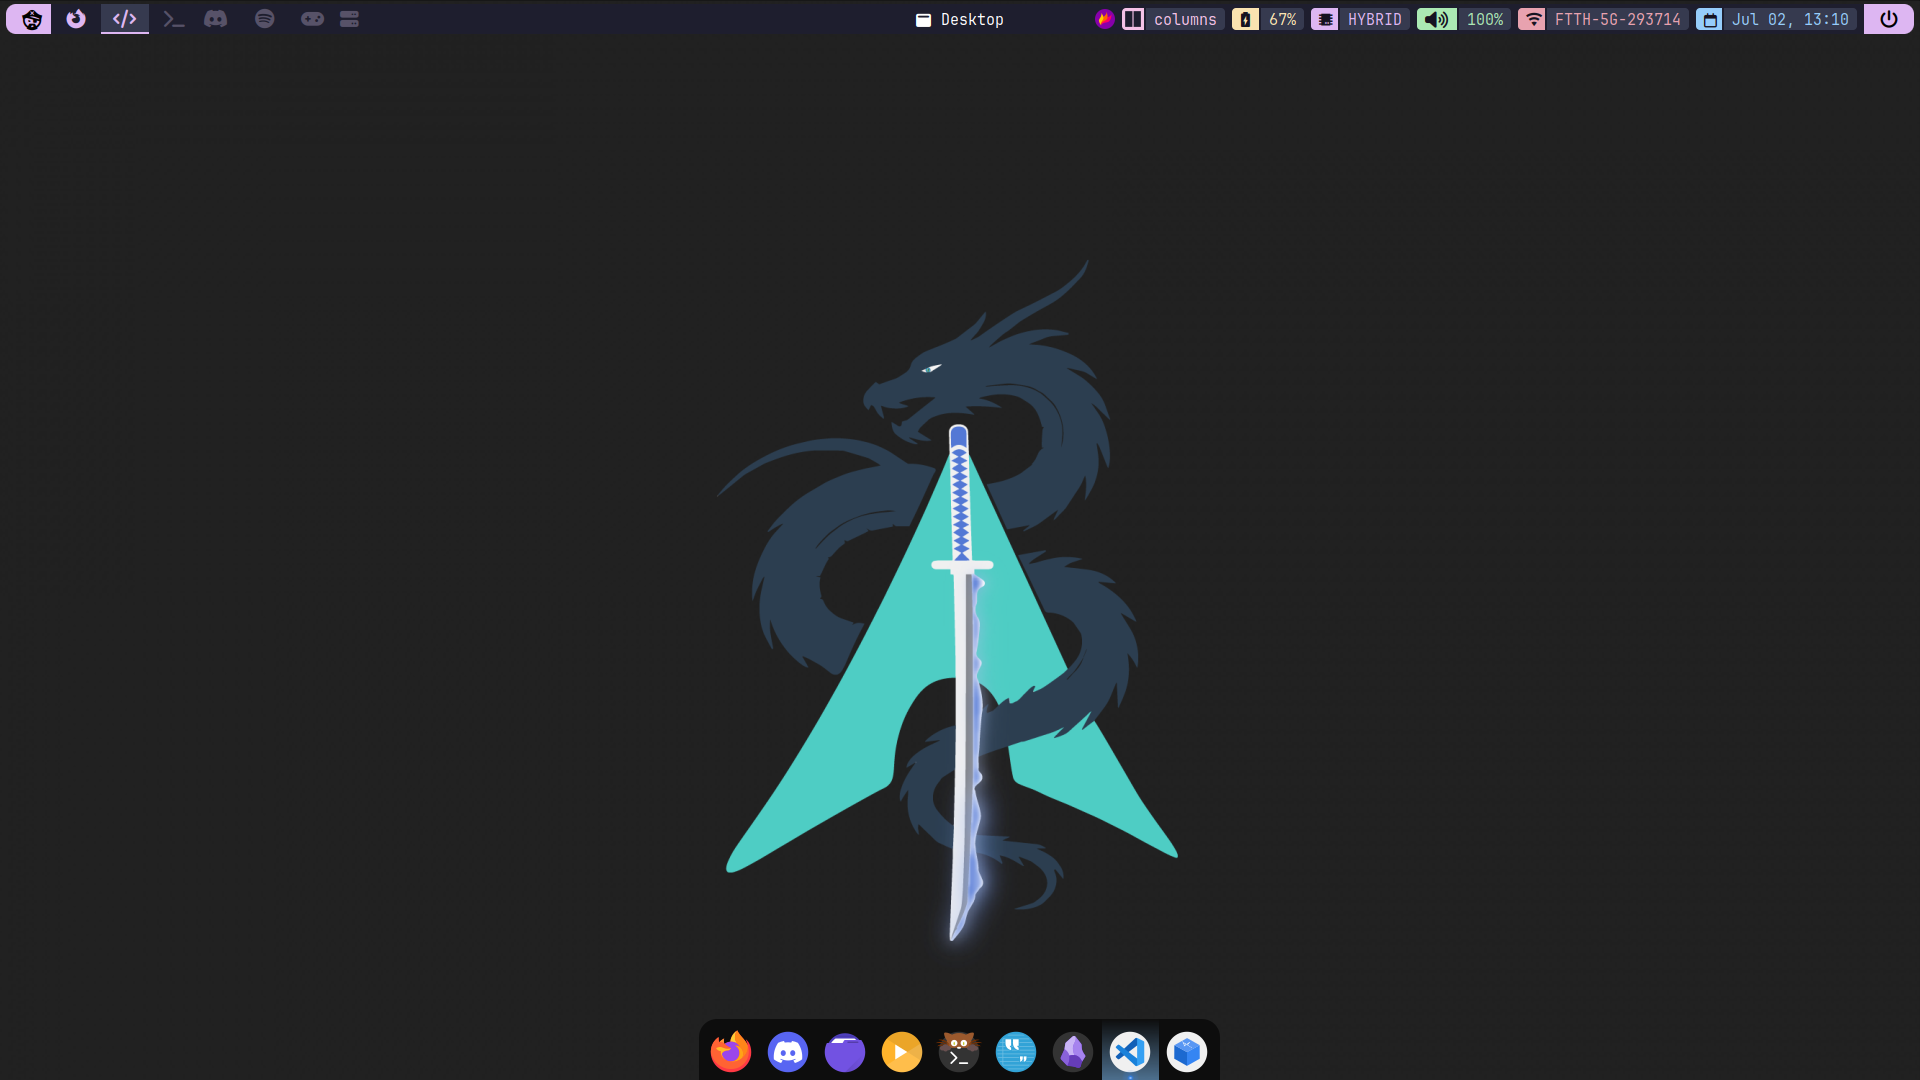
\includegraphics[width=0.9\textwidth]{images/desktop.png}
\caption{KyOS Desktop Environment featuring Qtile window manager with professional dark theme}
\end{figure}

\subsection{Design Philosophy}
The development of KyOS is guided by a philosophy that prioritizes security without sacrificing usability or performance. Every component included in the distribution undergoes security evaluation, ensuring that users receive a system designed with threats and vulnerabilities in mind from the ground up. This security-first approach doesn't mean complexity - instead, KyOS embraces a dual-purpose design that serves both daily computer users seeking a reliable, secure desktop experience and cybersecurity professionals requiring specialized tools and workflows.

The distribution follows a minimal bloat principle, including only essential components by default while providing extensive customization options during installation. This approach allows users to build exactly the system they need without unnecessary software consuming resources or expanding the attack surface. KyOS leverages modern architecture and contemporary technologies, ensuring users benefit from the latest security enhancements, performance optimizations, and software features available in the open-source ecosystem.

\subsection{Target Audience}
KyOS serves a broad spectrum of users, from everyday desktop users to specialized cybersecurity professionals. The distribution is designed to accommodate different skill levels and use cases while maintaining a consistent, secure foundation.

\textbf{Primary Users:}
Daily desktop users form a significant portion of KyOS's target audience, including those seeking a secure and efficient Linux experience without the complexity often associated with security-focused distributions. Students and hobbyists interested in learning cybersecurity find KyOS an ideal platform because it provides access to professional-grade tools in a stable, educational environment. Developers requiring a robust development environment benefit from the distribution's rolling-release model and comprehensive package availability, while privacy-conscious users appreciate the enhanced security features and minimal data collection inherent in the system design.

\textbf{Professional Users:}
The professional user base includes cybersecurity professionals and ethical hackers who require immediate access to cutting-edge security tools and a stable platform for conducting security assessments. System administrators and DevOps engineers utilize KyOS for security-hardened system administration and continuous security integration workflows. Security researchers and penetration testers benefit from the comprehensive tool selection and customizable environment that supports complex research methodologies. IT professionals requiring specialized security tools find KyOS provides a cohesive platform that eliminates the need to cobble together tools from multiple sources. Educational institutions teaching cybersecurity and system administration use KyOS as a standardized platform that students can use both in academic settings and professional environments.

\section{Technical Foundations}

\subsection{Arch Linux Foundation}

\subsubsection{The Arch Way}
Arch Linux follows a philosophy known as "The Arch Way," which emphasizes simplicity, modernity, pragmatism, user-centricity, and versatility. KyOS inherits these principles while adding specialized security and professional workflow enhancements.

The core Arch Linux principles that KyOS extends include maintaining simplicity by avoiding unnecessary modifications to upstream software, implementing cutting-edge features while keeping software packages current, focusing on practical solutions over ideological considerations, and designing for competent Linux users who value control over their system. KyOS builds upon this foundation by adding a general-purpose base system with unlimited customization potential, making it suitable for both daily use and specialized security work.

\subsubsection{Rolling Release Model}
Arch Linux employs a rolling release model, which KyOS inherits and extends. Unlike traditional distributions that release major versions periodically (like Ubuntu's 6-month cycle), rolling release systems continuously update software packages as new versions become available. This means users always have access to the latest software without waiting for major distribution releases.

The rolling release architecture flows from upstream sources through Arch repositories to KyOS integration. New software releases undergo testing phases and security reviews before reaching users through community quality assurance and professional validation processes. This results in stable, continuously updated systems that benefit security professionals and daily users alike.

For security professionals, rolling release provides immediate access to the newest security tools, rapid deployment of critical security patches, latest kernel features for hardware support, and eliminates version fragmentation across different installations. Daily users benefit from always having current software, automatic security updates, and access to the latest application features without complex upgrade procedures.

\subsubsection{Package Management}
Arch Linux's pacman package manager provides the foundation for KyOS package management:

\begin{lstlisting}[caption=Pacman Package Management Features]
# Core pacman functionality
pacman -S package_name     # Install package
pacman -R package_name     # Remove package
pacman -Syu               # System update
pacman -Ss search_term    # Search packages
pacman -Qi package_name   # Package information

# Advanced features used by KyOS
pacman -Qdt               # Find orphaned packages
pacman -U package.tar.xz  # Install local package
pacman -Sw package_name   # Download only
\end{lstlisting}

\subsection{Archiso Build System}

\subsubsection{ISO Creation Framework}
Archiso is the official tool for creating Arch Linux live media, which KyOS extends for custom distribution creation. Think of Archiso as a framework that takes a base Arch Linux system and packages it into a bootable ISO file that can be written to USB drives or DVDs.

\begin{figure}[H]
\centering
\begin{lstlisting}[caption=Archiso Build Process]
Base Configuration
    |-- profiledef.sh (Build configuration)
    |-- packages.x86_64 (Package list)
    |-- airootfs/ (Root filesystem overlay)
    |   |-- etc/ (System configuration)
    |   |-- usr/ (User programs and scripts)
    |   `-- root/ (Root user customizations)
    |-- efiboot/ (UEFI boot configuration)
    |-- grub/ (GRUB boot configuration)
    `-- syslinux/ (Legacy boot configuration)
\end{lstlisting}
\caption{Archiso Directory Structure}
\end{figure}

\subsubsection{KyOS Archiso Customizations}
KyOS implements several specialized customizations to the standard Archiso framework, including curated package selections for security and professional tools, branded boot loaders with KyOS theming for GRUB and syslinux, optimized systemd services and startup configurations, default security configurations with hardened settings, and pre-installed development and security tools for immediate productivity.

\subsubsection{Multi-Variant ISO Distribution}
KyOS addresses diverse hardware and virtualization requirements through three specialized ISO variants, each optimized for specific deployment scenarios:

\textbf{VirtualBox ISO:} Specifically configured for VirtualBox virtualized environments, this variant includes VirtualBox Guest Additions for optimal integration, modified Picom compositor settings optimized for virtual GPU performance, and hardware-specific drivers suitable for virtualized graphics acceleration. The VirtualBox variant eliminates compatibility issues common in virtualized environments and provides seamless clipboard integration, dynamic resolution adjustment, and optimized resource utilization for virtual machine deployment.

\textbf{Standard User ISO:} Designed for typical desktop and laptop hardware configurations, this variant includes comprehensive driver support for common hardware components, default Picom settings optimized for standard integrated and discrete graphics, and balanced performance configurations suitable for most daily computing scenarios. The standard variant provides excellent compatibility across diverse hardware manufacturers while maintaining optimal performance for both productivity and security workflows.

\textbf{NVIDIA User ISO:} Engineered specifically for systems with NVIDIA graphics hardware, this variant includes pre-installed NVIDIA proprietary drivers, optimized kernel modules for NVIDIA hardware acceleration, Picom configuration tuned for NVIDIA GPU capabilities, and specialized tools for NVIDIA graphics management. This variant eliminates the complexity typically associated with NVIDIA driver installation on Linux systems, providing users with immediate access to hardware acceleration, CUDA support for security tools requiring GPU computation, and optimized graphics performance for security visualization tools.

\subsection{Display Server Architecture}

\subsubsection{X11 Display Server}
KyOS utilizes the X11 display server (specifically X.Org Server) as its primary display system. The display server is the fundamental software component that manages your computer's graphics output, handles input from keyboard and mouse, and provides the foundation for all graphical applications to run.

While Wayland represents the newer generation of Linux display protocols and offers some technical improvements, X11 remains the preferred choice for KyOS due to several practical considerations. Many security and penetration testing tools were designed for X11 and may not work properly with Wayland. X11 provides superior support for remote access through SSH X11 forwarding, allowing users to run graphical security tools on remote servers. The protocol also offers excellent compatibility with screen sharing tools like VNC and NoMachine, which are essential for collaborative security work and remote administration.

Additionally, X11 benefits from decades of optimization and compatibility testing across diverse hardware configurations. The mature ecosystem includes extensive documentation, troubleshooting resources, and a wide selection of compatible window managers, giving users more choice in customizing their desktop environment.

\begin{lstlisting}[caption=X11 Architecture Components]
# X11 Server Components
X.Org Server
    |-- Input Drivers (keyboard, mouse, touchpad)
    |-- Video Drivers (Intel, AMD, NVIDIA)
    |-- Extensions (Composite, Render, XInput)
    `-- Protocol Handler (X11 protocol communication)

# KyOS X11 Configuration
/etc/X11/
    |-- xorg.conf.d/
    |   |-- 20-intel.conf
    |   |-- 20-amd.conf
    |   `-- 20-nvidia.conf
    `-- xinit/
        `-- xinitrc (Session startup)
\end{lstlisting}

\subsubsection{Display Server vs. Window Manager vs. Display Manager}

To clarify the relationship between these components in KyOS:

\textbf{Display Server (X11):}
The X11 display server serves as the fundamental layer that enables graphical interfaces on Linux systems. Think of it as the communication bridge between software applications and your computer's graphics hardware. X11 handles the low-level operations like drawing pixels on screen, managing mouse and keyboard input, and communicating with graphics cards. What makes X11 particularly powerful is its network-transparent design, meaning you can run applications on one computer while displaying them on another across a network - a feature that proves invaluable for remote security testing and system administration.

\textbf{Window Manager (Qtile):}
The window manager controls how graphical applications appear and behave on your screen. While the display server handles the basic graphics, the window manager decides where windows are positioned, how they can be resized, and how users interact with them. Qtile specifically uses a "tiling" approach, which means windows automatically arrange themselves to fill the screen efficiently without overlapping. This eliminates the need to manually resize and position windows, creating a more organized workspace where every application is visible and accessible.

\textbf{Display Manager (SDDM):}
The display manager is what you see when you first boot into a graphical system - it's the login screen that appears before you enter your desktop environment. SDDM (Simple Desktop Display Manager) handles user authentication, session management, and provides the interface for selecting which desktop environment or window manager to use. Once you log in, SDDM starts your chosen session (in KyOS's case, the Qtile window manager) and then steps aside to let you work.

\begin{figure}[H]
\centering
\begin{lstlisting}[caption=KyOS Display Stack]
User Applications
        |
        v
Qtile Window Manager
        |
        v
X11 Display Server
        |
        v
GPU Drivers (Intel/AMD/NVIDIA)
        |
        v
Hardware (Graphics Card)

Login Flow:
SDDM Display Manager --> User Authentication --> Qtile Session Start
\end{lstlisting}
\caption{KyOS Display Architecture Stack}
\end{figure}

\subsection{Qtile Window Manager}

\subsubsection{Why Qtile for All Users}
KyOS employs Qtile as its default window manager, chosen for its advantages across different user types:

\textbf{Benefits for Daily Users:}
Qtile offers daily users an efficient workflow centered around keyboard shortcuts, significantly reducing the time spent manually arranging windows and switching between applications. The window manager's Python-based configuration system provides extensive customization options, allowing users to personalize their desktop environment without learning complex configuration languages. Despite its powerful features, Qtile maintains excellent resource efficiency, consuming significantly less memory than traditional desktop environments like GNOME or KDE, leaving more system resources available for applications and multitasking.

For users new to tiling window managers, Qtile serves as an excellent learning opportunity, introducing concepts that improve productivity and workflow efficiency once mastered. The distraction-free environment helps maintain focus during work and study sessions by eliminating visual clutter and providing organized workspaces. Multi-monitor support is exceptionally well-implemented, making Qtile an excellent choice for users with complex display setups commonly found in development, content creation, and professional workflows.

\textbf{Additional Benefits for Security Professionals:}
Security professionals benefit from Qtile's terminal-centric design, which optimizes the workflow for command-line security tools that form the backbone of most security operations. Quick navigation between workspaces allows professionals to organize different aspects of security assessments (reconnaissance, exploitation, documentation) into separate, instantly accessible areas. The window manager excels at multi-tasking scenarios where multiple security tools need to run simultaneously while maintaining visibility and easy switching between applications.

Qtile's automation capabilities allow security professionals to script window and workspace management, creating reproducible work environments for different types of security assessments. The professional workflow optimization includes layouts specifically designed for security analysis tasks, such as having terminal windows for tool execution alongside web browsers for research and documentation tools for reporting.

\begin{lstlisting}[caption=Qtile Configuration Example]
# KyOS Qtile Configuration
from libqtile import bar, layout, widget
from libqtile.config import Click, Drag, Group, Key, Match, Screen
from libqtile.lazy import lazy

# KyOS-specific key bindings
keys = [
    # Security tool shortcuts
    Key([mod], "t", lazy.spawn("alacritty")),
    Key([mod], "w", lazy.spawn("firefox")),
    Key([mod], "n", lazy.spawn("nmap-gui")),
    Key([mod], "b", lazy.spawn("burpsuite")),
    
    # Workspace management for security workflows
    Key([mod], "1", lazy.group["web"].toscreen()),
    Key([mod], "2", lazy.group["recon"].toscreen()),
    Key([mod], "3", lazy.group["exploitation"].toscreen()),
    Key([mod], "4", lazy.group["reporting"].toscreen()),
]

# Professional workspace groups
groups = [
    Group("web", label="Web Analysis"),
    Group("recon", label="Reconnaissance"),
    Group("exploitation", label="Exploitation"),
    Group("reporting", label="Documentation"),
]
\end{lstlisting}

\subsubsection{Tiling Window Management Philosophy}
Tiling window managers like Qtile represent a fundamental shift from the traditional "floating" window approach used by most desktop environments. Instead of windows that can overlap and hide each other, tiling managers automatically arrange windows in non-overlapping layouts that utilize every pixel of available screen space. This approach provides several significant advantages, particularly for security professionals who often need to monitor multiple tools and data streams simultaneously.

The spatial efficiency of tiling eliminates wasted screen real estate and ensures that information is always visible without requiring constant window switching or Alt-Tab navigation. This visibility reduces cognitive load because users don't need to remember what applications are running behind other windows or mentally track window positions. The predefined layouts optimize common workflow patterns, such as having a main application window with supporting tool windows arranged around it.

For security professionals, the ability to coordinate multiple tools becomes particularly valuable during complex assessments where reconnaissance tools, exploitation frameworks, and documentation applications need to be visible and accessible simultaneously. Unlike traditional desktop environments where security professionals might struggle with overlapping terminal windows and hidden applications, tiling window management ensures that all relevant tools remain visible and organized throughout the assessment process.

\begin{figure}[H]
\centering
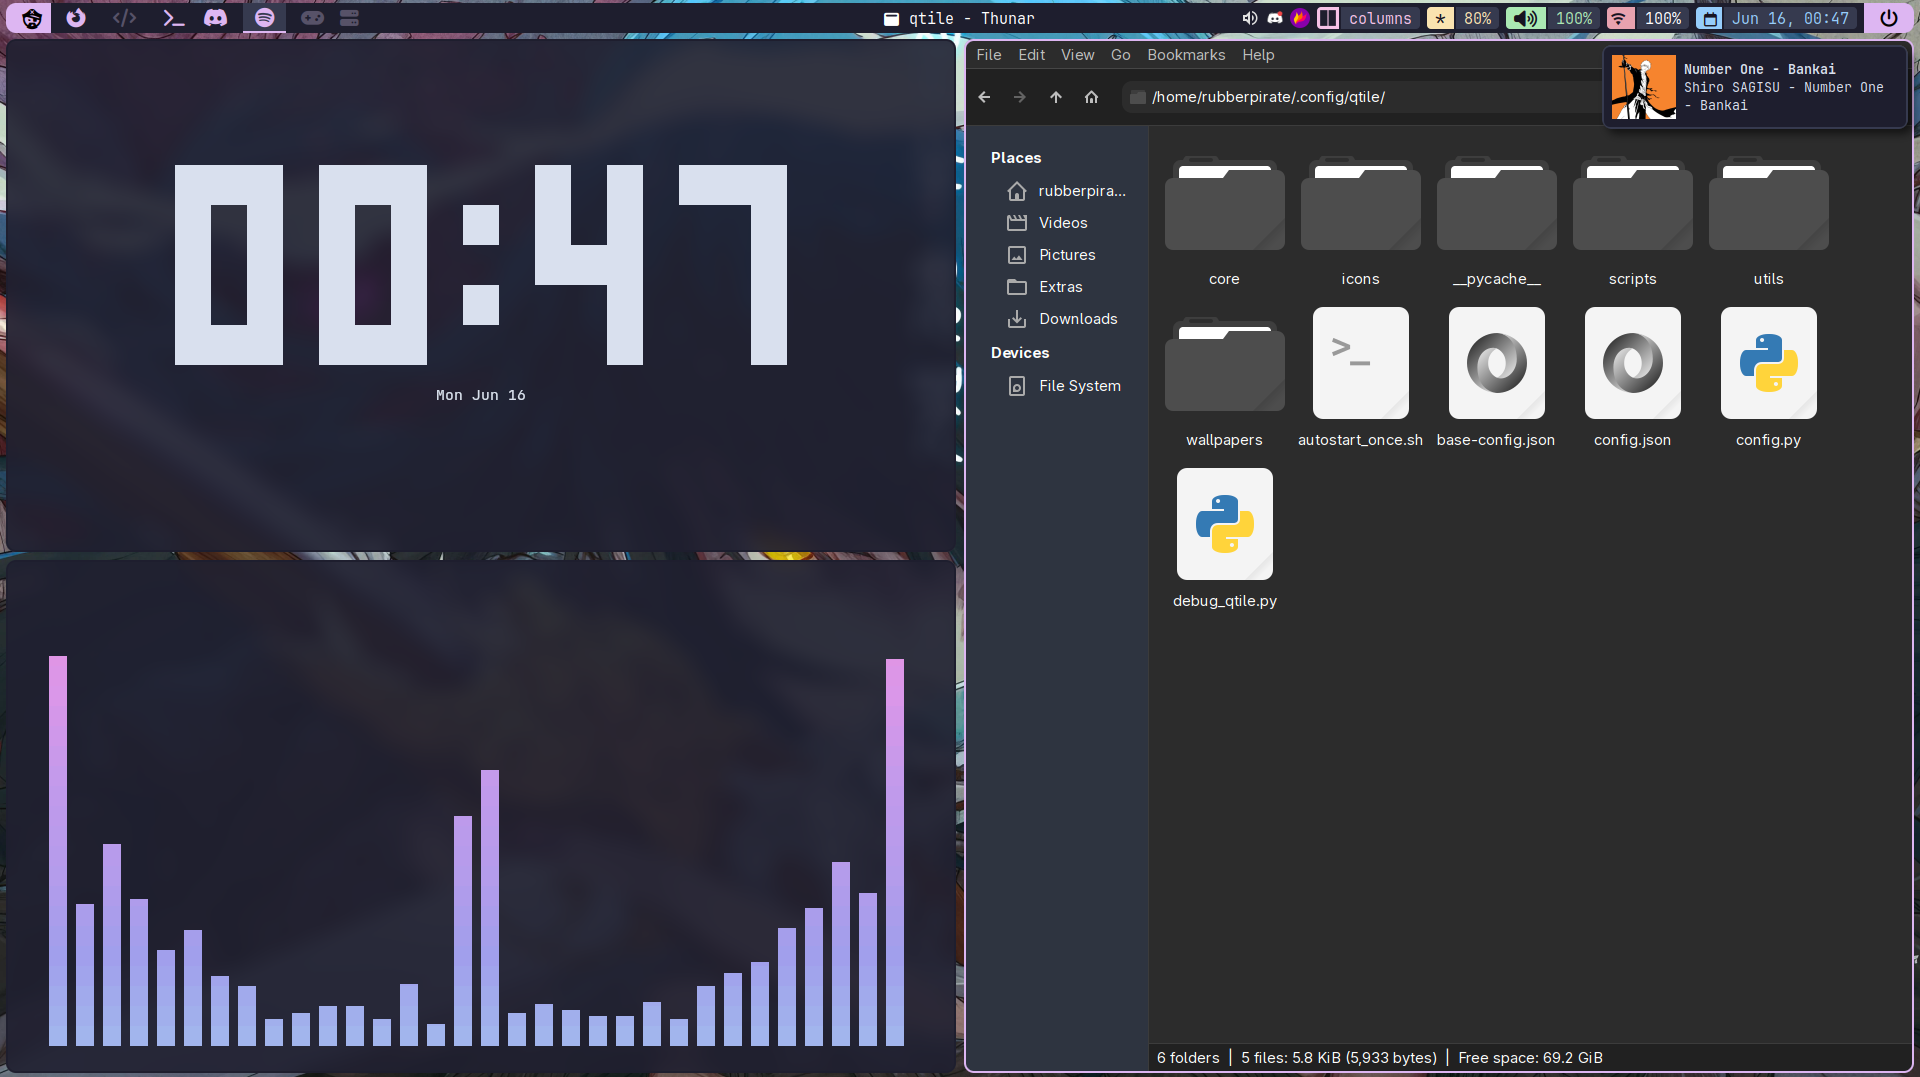
\includegraphics[width=0.9\textwidth]{images/tilling_windows.png}
\caption{Qtile Tiling Window Management - Multiple applications arranged efficiently without overlap}
\end{figure}

For comparison with traditional window management approaches, floating window managers allow windows to overlap and be positioned manually by the user. While this approach offers flexibility in window placement, it can lead to visual clutter and reduced efficiency, particularly in professional workflows requiring simultaneous access to multiple tools.

\begin{figure}[H]
\centering
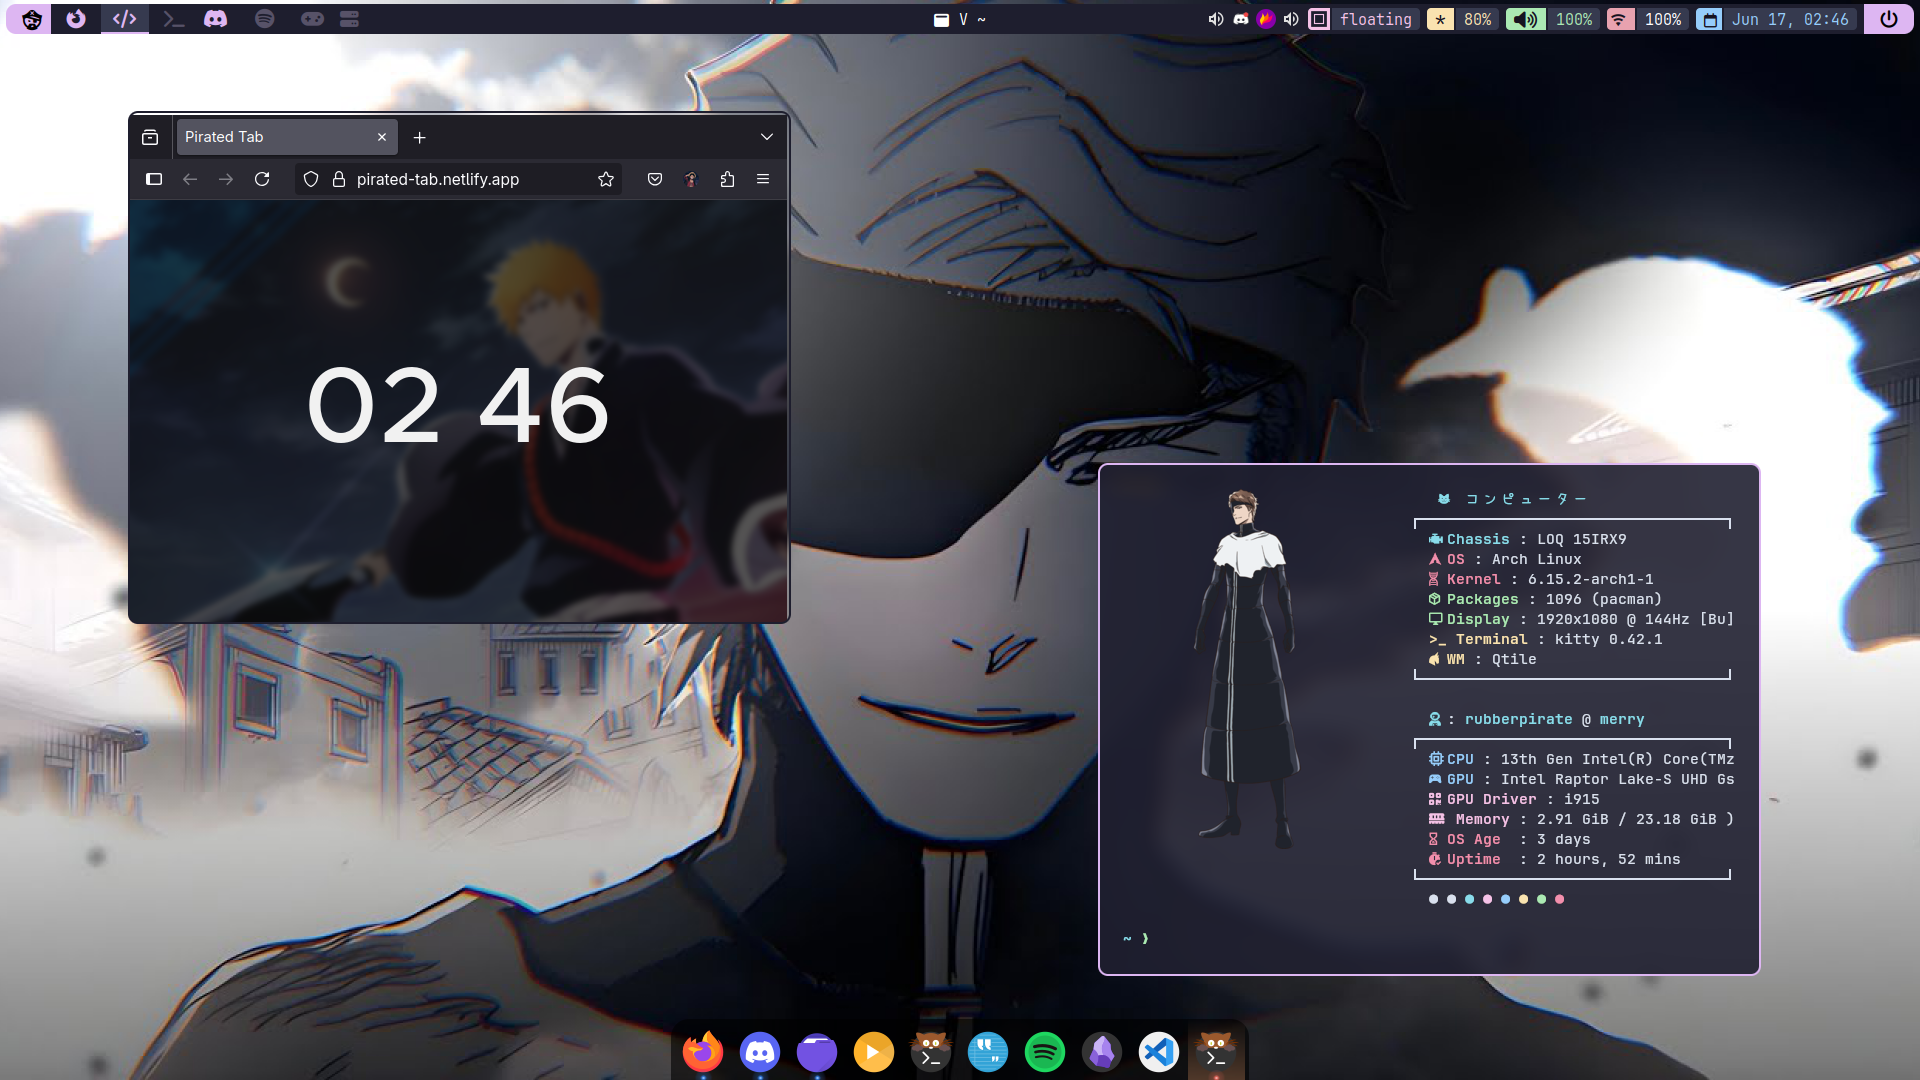
\includegraphics[width=0.9\textwidth]{images/floating_windows.png}
\caption{Traditional Floating Window Management - Windows can overlap and hide content}
\end{figure}

\begin{table}[H]
\centering
\begin{tabular}{@{}lll@{}}
\toprule
\textbf{Layout Type} & \textbf{Use Case} & \textbf{Security Application} \\
\midrule
Tall & Main + Support & Terminal + Documentation \\
Max & Single Focus & Full-screen analysis tools \\
Matrix & Grid Organization & Multiple monitoring terminals \\
MonadWide & Wide Main & Web app testing + tools \\
Floating & Traditional & Legacy security applications \\
\bottomrule
\end{tabular}
\caption{Qtile Layout Applications in Security Work}
\end{table}

\subsection{KyOS Purpose and Target Applications}

\subsubsection{Daily Computing Use Cases}
KyOS serves as an excellent daily driver operating system, providing enhanced security features without sacrificing the usability expected in modern desktop environments.

\textbf{Personal Computing and Productivity:}
The distribution provides a secure daily desktop environment with built-in privacy features that protect user data without requiring extensive configuration knowledge. As a development workstation, KyOS offers comprehensive programming tools and environments suitable for software development across multiple languages and frameworks. Content creators benefit from professional-grade tools integrated into a stable, performance-optimized platform that handles resource-intensive applications effectively.

Educational users find KyOS particularly valuable as a learning environment for both Linux system administration and cybersecurity concepts. The distribution serves as a bridge between general-purpose computing and specialized security work, allowing students to gradually build expertise while using the same tools they'll encounter in professional environments. Privacy-conscious users appreciate the distribution's approach to web browsing and communication, which prioritizes user privacy through secure defaults and minimal data collection.

\textbf{Academic and Learning Applications:}
Educational institutions utilize KyOS as a comprehensive platform for computer science and cybersecurity education, providing students with hands-on experience using professional-grade security tools in a controlled, safe environment. The distribution creates an ideal learning environment for Linux system administration, allowing students to experiment with system configuration and management without the complexity of building a system from scratch.

Security tool experimentation becomes accessible and safe within KyOS, providing students with supervised access to the same tools used by professional security practitioners. Programming and development skills practice benefits from the distribution's comprehensive development environment and access to modern programming languages and frameworks. Research and academic project development find strong support through KyOS's combination of stability, cutting-edge software availability, and comprehensive documentation.

\subsubsection{Professional Security Use Cases}
KyOS is specifically engineered for critical cybersecurity applications:

\subsubsection{Professional Security Use Cases}
KyOS is specifically engineered for critical cybersecurity applications, providing professionals with a comprehensive platform that supports the full spectrum of security operations.

\textbf{Penetration Testing and Ethical Hacking:}
Red team operations and adversary simulation benefit from KyOS's comprehensive tool selection and stable platform that supports long-duration assessments without system instability. Web application security assessment becomes more efficient through integrated tools and workflows designed specifically for web security testing methodologies. Network penetration testing and vulnerability assessment operations leverage the distribution's network analysis capabilities and automated scanning tools.

Wireless security auditing and testing receive dedicated support through specialized wireless tools and drivers that handle a wide range of wireless hardware and protocols. Social engineering assessment platforms benefit from the distribution's ability to create realistic test environments and communication tools necessary for authorized social engineering assessments.

\textbf{Security Research and Analysis:}
Malware analysis and reverse engineering operations utilize KyOS's isolated environment capabilities and specialized analysis tools that allow researchers to safely examine suspicious software without risking system compromise. Cryptographic research and analysis benefit from the distribution's mathematical and cryptographic libraries alongside development tools for creating and testing cryptographic implementations.

Security tool development and testing find comprehensive support through the distribution's development environment and testing frameworks. Vulnerability research and discovery operations leverage the platform's stability and tool availability for systematic security research methodologies. Security automation and scripting benefit from the Python-based configuration system and extensive scripting language support throughout the distribution.

\textbf{Digital Forensics and Incident Response:}
Digital forensics investigations utilize KyOS as a comprehensive investigation platform with tools for examining various types of digital evidence while maintaining chain of custody requirements. Incident response toolkit deployment benefits from the distribution's rapid deployment capabilities and comprehensive incident response tool collection.

Memory analysis and artifact examination leverage specialized forensics tools integrated into the distribution alongside the computational power necessary for complex forensics operations. Network forensics and traffic analysis operations utilize advanced network analysis tools and large-scale data processing capabilities. Mobile device forensics capabilities extend the platform's forensics reach to modern mobile devices and embedded systems.

\textbf{System Administration and DevSecOps:}
Security-hardened system administration benefits from KyOS's secure defaults and comprehensive administrative tools that allow administrators to maintain security while managing complex systems. Continuous security integration (DevSecOps) workflows find support through automated security testing tools and integration frameworks that embed security testing into development pipelines.

Infrastructure security monitoring utilizes the distribution's monitoring tools and alerting systems to maintain situational awareness of large-scale infrastructure security. Compliance auditing and reporting benefit from automated compliance checking tools and comprehensive reporting capabilities. Security automation and orchestration leverage the platform's scripting capabilities and tool integration to create comprehensive security automation workflows.

\subsubsection{Educational and Training Applications}
KyOS serves as an exceptional platform for cybersecurity education, providing students and professionals with hands-on experience using the same tools and environments they will encounter in their careers. Academic institutions integrate KyOS into cybersecurity curricula, offering students practical experience with professional-grade security tools in a controlled educational environment. This approach bridges the gap between theoretical knowledge and practical application, preparing students for real-world security challenges.

Professional training programs utilize KyOS for hands-on security training labs, where students can practice security techniques and tool usage in realistic scenarios without the risks associated with live environments. The distribution provides an ideal platform for certification preparation, particularly for hands-on certifications like OSCP (Offensive Security Certified Professional), CEH (Certified Ethical Hacker), and CISSP (Certified Information Systems Security Professional) lab environments.

Capture The Flag (CTF) competitions and practice environments benefit from KyOS's comprehensive tool selection and stable platform that can handle the intense computational demands of competitive security challenges. Graduate-level security research projects find strong support through the distribution's research-oriented tools and academic resources, allowing students to conduct sophisticated security research within a well-supported environment.

\section{System Architecture}

\subsection{Core Components}

\subsubsection{Base System}
KyOS utilizes Arch Linux as its foundation, inheriting the powerful characteristics that make Arch Linux a preferred choice for advanced users and system administrators. The rolling release model ensures users always have access to the latest software versions without waiting for major distribution releases, providing immediate access to security patches, bug fixes, and new features as they become available upstream.

The Pacman package manager, combined with access to the Arch User Repository (AUR), provides users with one of the most comprehensive software repositories in the Linux ecosystem. This combination allows users to install both officially maintained packages and community-contributed software through a unified interface. The systemd init system provides modern service management capabilities, including parallel service startup, dependency-based service management, and comprehensive logging through journald.

The modern kernel foundation includes the latest security patches and hardware support, ensuring compatibility with contemporary hardware while maintaining security against newly discovered vulnerabilities. Regular kernel updates provide access to performance improvements, new hardware drivers, and enhanced security features as they become available from the Linux kernel development community.

\subsubsection{Desktop Environment}
The default desktop environment represents a carefully balanced approach between functionality and efficiency, designed to support both daily users and security professionals without overwhelming system resources.

Qtile serves as the Python-based tiling window manager, providing users with a highly customizable and programmable interface that can be adapted to individual workflows and preferences. The Python configuration system allows users to create sophisticated window management behaviors and integrate external tools and scripts directly into their desktop environment.

Professional dark theming with KyOS branding creates a cohesive visual experience that reduces eye strain during extended work sessions, particularly important for security professionals who often work in low-light environments or during extended analysis sessions. The keyboard-driven interface design optimizes workflow efficiency by reducing reliance on mouse interactions, allowing users to maintain focus on their work without frequent context switching between keyboard and mouse.

Resource efficiency remains a priority throughout the desktop environment, with careful attention paid to memory usage and CPU consumption to ensure maximum system resources remain available for user applications and security tools. This efficiency becomes particularly important when running resource-intensive security tools or analyzing large datasets.

\subsection{Installation System Architecture}

\subsubsection{Unified Installer Design}
The KyOS installation system consists of several interconnected components:

\begin{figure}[H]
\centering
\begin{lstlisting}[caption=Installation System Components]
kyos-install (Main TUI Interface)
    |-- Interactive Mode
    |   |-- Configuration Wizard
    |   |-- Hardware Detection
    |   `-- Feature Selection
    |-- Automated Mode
    |   |-- Quick Installation
    |   `-- Sensible Defaults
    `-- Backend Integration
        |-- kyosinstall-auto (Core Logic)
        |-- Configuration Management
        `-- Error Handling
\end{lstlisting}
\caption{KyOS Installation System Architecture}
\end{figure}

\subsubsection{Installation Workflow}
The installation process follows a structured workflow:

\begin{enumerate}
    \item \textbf{Pre-installation:} System verification and preparation
    \item \textbf{Configuration:} User preferences and system settings
    \item \textbf{Partitioning:} Disk layout and filesystem selection
    \item \textbf{Base Installation:} Core system installation
    \item \textbf{Feature Installation:} Optional components and tools
    \item \textbf{Post-installation:} System finalization and optimization
\end{enumerate}

\section{Installation System Implementation}

\subsection{Text User Interface (TUI)}

\subsubsection{Design Principles}
The TUI installer implements carefully considered design principles that prioritize user experience and reduce installation complexity. Intuitive navigation utilizes clear menu structures and logical flow patterns that guide users through the installation process without confusion or ambiguity. Each step in the installation process follows naturally from the previous step, creating a coherent experience that doesn't require users to understand the underlying technical complexity.

Professional appearance maintains consistent branding and styling throughout the installation process, creating a polished experience that reflects the quality and attention to detail users can expect from the completed system. The visual design choices support rather than distract from the installation tasks, using color and typography strategically to highlight important information and guide user attention.

Error prevention becomes critical during system installation where mistakes can result in data loss or failed installations. The installer implements comprehensive input validation that checks user entries for correctness before proceeding, confirmation dialogs for potentially destructive actions, and clear error messages that help users understand and correct problems when they occur.

Accessibility support ensures that users with different needs and preferences can successfully complete installations. Keyboard-only navigation support allows users who cannot or prefer not to use pointing devices to access all installer functionality, while clear visual hierarchies and readable fonts support users with visual impairments.

\subsubsection{Implementation Details}
\begin{lstlisting}[caption=TUI Implementation Example]
#!/bin/bash
# KyOS TUI Installer Implementation

# Color scheme and branding
KYOS_BLUE="#1E90FF"
KYOS_GREEN="#00FF7F"
KYOS_RED="#FF4500"

# Main installer function
show_main_menu() {
    gum choose --header="KyOS Installation System" \
               --selected.foreground="$KYOS_BLUE" \
               "Install KyOS" \
               "Configure Options" \
               "Hardware Detection" \
               "Exit"
}

# Configuration management
save_config() {
    cat > /tmp/kyos-config << EOF
HOSTNAME="$hostname"
USERNAME="$username"
BLACKARCH="$blackarch_support"
NVIDIA="$nvidia_support"
SWAP_TYPE="$swap_type"
EOF
}
\end{lstlisting}

\subsection{Hardware Detection and Optimization}

\subsubsection{NVIDIA Graphics Support}
KyOS includes comprehensive NVIDIA graphics support:

\begin{lstlisting}[caption=NVIDIA Detection and Installation]
install_nvidia_drivers() {
    print_info "Installing NVIDIA drivers and utilities..."
    
    # Detect kernel type for proper driver selection
    case "$kernel" in
        "linux")     kernel_pkg="nvidia-dkms" ;;
        "linux-lts") kernel_pkg="nvidia-dkms" ;;
        "linux-zen") kernel_pkg="nvidia-dkms" ;;
        *)           kernel_pkg="nvidia-dkms" ;;
    esac
    
    # Install NVIDIA drivers and utilities
    arch-chroot /mnt pacman -S --noconfirm \
        $kernel_pkg nvidia-utils nvidia-settings \
        opencl-nvidia libva-nvidia-driver
    
    # Configure kernel modules
    sed -i 's/^MODULES=(\(.*\))/MODULES=(\1 nvidia nvidia_modeset nvidia_uvm nvidia_drm)/' \
        /mnt/etc/mkinitcpio.conf
    
    # Add kernel parameters
    sed -i 's/GRUB_CMDLINE_LINUX_DEFAULT="\(.*\)"/GRUB_CMDLINE_LINUX_DEFAULT="\1 nvidia-drm.modeset=1"/' \
        /mnt/etc/default/grub
}
\end{lstlisting}

\subsubsection{Memory Management}
KyOS implements advanced memory management through ZRAM:

\begin{lstlisting}[caption=ZRAM Configuration]
setup_zram() {
    print_info "Setting up ZRAM compressed swap..."
    
    # Create ZRAM configuration
    cat > /mnt/etc/systemd/zram-generator.conf << EOF
[zram0]
zram-size = ram / 2
compression-algorithm = zstd
swap-priority = 100
fs-type = swap
EOF
    
    # Enable ZRAM service
    arch-chroot /mnt systemctl enable systemd-zram-setup@zram0.service
}
\end{lstlisting}

\section{User Experience and Accessibility}

\subsection{Daily User Experience}

\subsubsection{User-Friendly Features}
While KyOS provides professional security capabilities, it maintains accessibility for daily users:

\textbf{Intuitive Installation:}
\begin{itemize}
    \item \textbf{Guided TUI Installer:} Step-by-step installation process with clear instructions
    \item \textbf{Automated Mode:} Quick installation with sensible defaults for beginners
    \item \textbf{Hardware Detection:} Automatic detection and configuration of common hardware
    \item \textbf{Help System:} Comprehensive help and documentation integrated into installer
\end{itemize}

\textbf{Desktop Environment:}
\begin{itemize}
    \item \textbf{Intuitive Shortcuts:} Common keyboard shortcuts for window management
    \item \textbf{Visual Indicators:} Clear status bars and system information displays
    \item \textbf{Application Menu:} Easy access to installed applications and tools
    \item \textbf{Customizable Themes:} Multiple color schemes and visual options
\end{itemize}

\subsubsection{Learning and Documentation}
KyOS includes comprehensive resources for users of all skill levels:

\textbf{Built-in Documentation:}
\begin{itemize}
    \item \textbf{Getting Started Guide:} Introduction to KyOS and basic usage
    \item \textbf{Qtile Tutorial:} Interactive guide to tiling window management
    \item \textbf{Security Tools Overview:} Introduction to available security tools
    \item \textbf{System Administration Guide:} Basic system maintenance and configuration
\end{itemize}

\textbf{Community Resources:}
\begin{itemize}
    \item \textbf{Online Documentation:} Comprehensive web-based documentation
    \item \textbf{Community Forums:} User support and discussion forums
    \item \textbf{Tutorial Videos:} Video guides for common tasks and workflows
    \item \textbf{Example Configurations:} Pre-made configurations for different use cases
\end{itemize}

\subsection{Accessibility Features}

\subsubsection{Universal Design}
KyOS implements accessibility features to ensure usability for all users:

\textbf{Visual Accessibility:}
\begin{itemize}
    \item \textbf{High Contrast Themes:} Multiple high-contrast color schemes
    \item \textbf{Font Scaling:} Adjustable font sizes throughout the interface
    \item \textbf{Screen Reader Support:} Compatibility with assistive technologies
    \item \textbf{Color Blind Friendly:} Color schemes designed for color vision deficiency
\end{itemize}

\textbf{Input Accessibility:}
\begin{itemize}
    \item \textbf{Keyboard Navigation:} Complete keyboard-only operation capability
    \item \textbf{Customizable Shortcuts:} User-definable keyboard shortcuts
    \item \textbf{Mouse Alternatives:} Support for alternative input devices
    \item \textbf{Voice Recognition:} Integration with speech recognition software
\end{itemize}

\section{Security Integration}

\subsection{BlackArch Repository Integration}

\subsubsection{Repository Management}
KyOS provides seamless integration with the BlackArch repository:

\begin{lstlisting}[caption=BlackArch Repository Setup]
install_blackarch() {
    print_info "Setting up BlackArch repository..."
    
    # Method 1: Official bootstrap
    if arch-chroot /mnt bash -c "
        curl -O https://blackarch.org/strap.sh
        chmod +x strap.sh
        ./strap.sh 2>/dev/null
        pacman -Syy --noconfirm
    "; then
        print_info "BlackArch repository setup completed!"
        return 0
    fi
    
    # Method 2: Manual fallback
    setup_blackarch_manual
}

setup_blackarch_manual() {
    # Download and install keyring
    curl -L -o blackarch-keyring.pkg.tar.zst \
        https://www.blackarch.org/keyring/blackarch-keyring.pkg.tar.zst
    
    arch-chroot /mnt pacman -U --noconfirm blackarch-keyring.pkg.tar.zst
    
    # Add repository to pacman.conf
    cat >> /mnt/etc/pacman.conf << EOF

[blackarch]
Server = https://www.blackarch.org/blackarch/\$repo/os/\$arch
EOF
    
    arch-chroot /mnt pacman -Syy
}
\end{lstlisting}

\subsubsection{Security Tool Categories}
BlackArch integration provides access to over 2600 security tools across categories:

\begin{figure}[H]
\centering
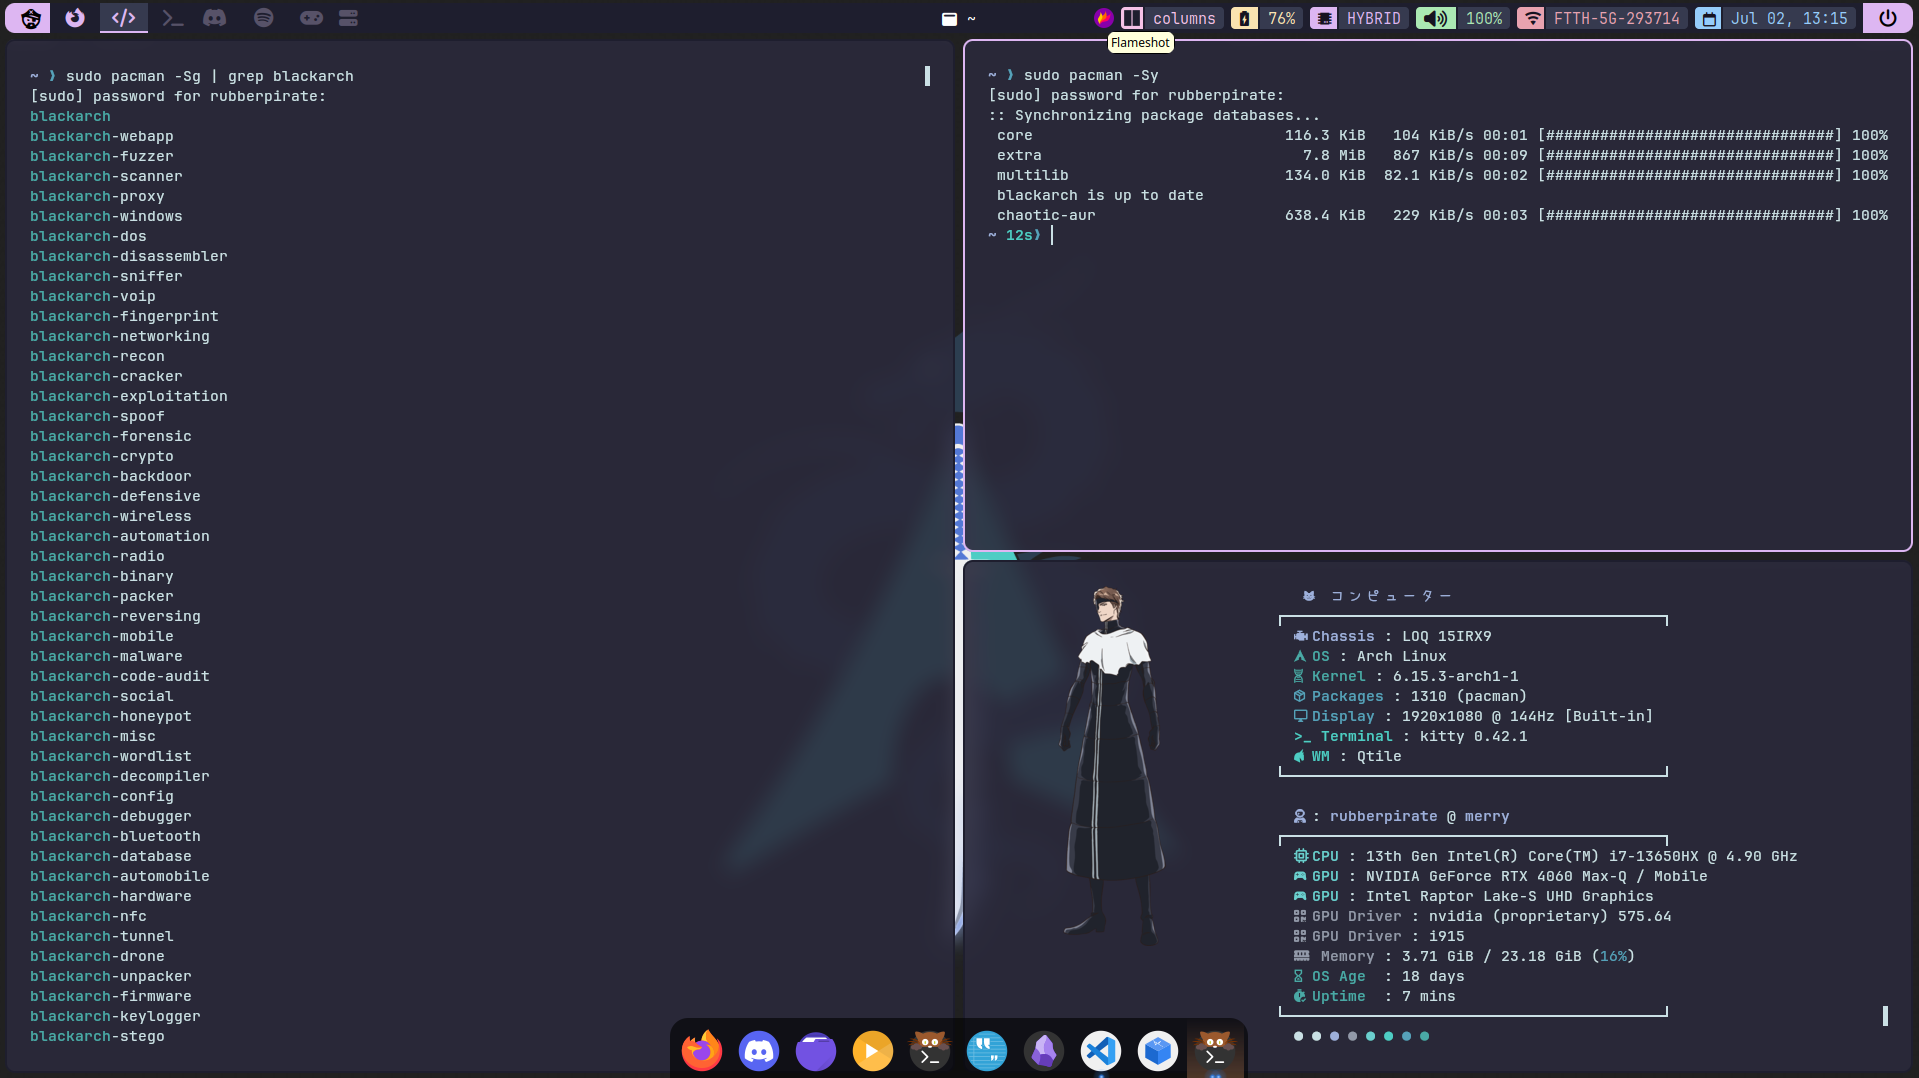
\includegraphics[width=0.9\textwidth]{images/terminal_packages_support.png}
\caption{KyOS Terminal Environment showing package management and security tool installation capabilities}
\end{figure}

\begin{table}[H]
\centering
\begin{tabular}{@{}ll@{}}
\toprule
\textbf{Category} & \textbf{Example Tools} \\
\midrule
Network Analysis & nmap, wireshark, masscan \\
Web Application & burpsuite, sqlmap, nikto \\
Wireless Security & aircrack-ng, reaver, kismet \\
Forensics & autopsy, sleuthkit, volatility \\
Exploitation & metasploit, exploit-db, searchsploit \\
Social Engineering & set, king-phisher, gophish \\
\bottomrule
\end{tabular}
\caption{BlackArch Tool Categories}
\end{table}

\subsection{System Hardening}

\subsubsection{Default Security Configurations}
KyOS implements several security hardening measures by default:

\begin{itemize}
    \item \textbf{Firewall:} UFW (Uncomplicated Firewall) enabled by default
    \item \textbf{SSH:} Secure SSH configuration with key-based authentication
    \item \textbf{User Permissions:} Proper sudo configuration and user groups
    \item \textbf{System Updates:} Automated security update notifications
\end{itemize}

\section{Performance Optimization}

\subsection{System Performance}

\subsubsection{Boot Optimization}
KyOS implements several boot-time optimizations:

\begin{lstlisting}[caption=Boot Optimization Configuration]
# Systemd optimization
systemd.analyze critical-chain
systemd.analyze blame

# Enable fast boot
echo 'FastBoot=true' >> /etc/systemd/system.conf

# Optimize initramfs
sed -i 's/^HOOKS=.*/HOOKS=(base udev autodetect modconf kms keyboard keymap consolefont block filesystems fsck)/' /etc/mkinitcpio.conf
\end{lstlisting}

\subsubsection{Memory Optimization}
\begin{itemize}
    \item \textbf{ZRAM:} Compressed swap in RAM
    \item \textbf{Kernel Parameters:} Optimized for performance
    \item \textbf{Service Management:} Minimal running services
    \item \textbf{Process Scheduling:} CPU scheduler optimization
\end{itemize}

\subsection{Storage Optimization}

\subsubsection{Filesystem Selection}
KyOS supports multiple filesystem options:

\begin{table}[H]
\centering
\begin{tabular}{@{}lll@{}}
\toprule
\textbf{Filesystem} & \textbf{Advantages} & \textbf{Use Case} \\
\midrule
Btrfs & Snapshots, compression & General use, development \\
Ext4 & Stability, compatibility & Production systems \\
XFS & High performance & Large files, databases \\
F2FS & SSD optimized & Mobile, embedded systems \\
\bottomrule
\end{tabular}
\caption{Supported Filesystems}
\end{table}

\section{Development Methodology}

\subsection{Version Control and Release Management}

\subsubsection{Development Workflow}
The KyOS development process follows a structured approach:

\begin{enumerate}
    \item \textbf{Feature Planning:} Requirements analysis and design
    \item \textbf{Implementation:} Code development and testing
    \item \textbf{Quality Assurance:} Comprehensive testing procedures
    \item \textbf{Integration:} Merging and compatibility verification
    \item \textbf{Release Preparation:} Documentation and packaging
    \item \textbf{Deployment:} Distribution and user support
\end{enumerate}

\subsubsection{Quality Assurance}
Quality assurance processes encompass multiple testing methodologies designed to ensure system reliability and security across diverse deployment scenarios. Automated testing forms the foundation of the quality assurance program, utilizing unit tests that verify individual component functionality and integration tests that validate how different system components work together under various conditions.

Manual testing procedures complement automated testing by conducting installation testing across various hardware configurations, ensuring that KyOS functions correctly on different processors, graphics cards, storage devices, and peripheral hardware. This hands-on testing reveals compatibility issues that automated testing might miss, particularly those related to hardware-specific behaviors and edge cases.

Security auditing represents a critical component of the quality assurance process, involving comprehensive code review procedures that examine all system components for potential security vulnerabilities. Security analysis extends beyond code review to include configuration validation, privilege assessment, and attack surface analysis to identify potential security risks before release.

Performance benchmarking validates system performance across different hardware configurations and usage scenarios, ensuring that KyOS delivers consistent performance whether deployed on high-end workstations or resource-constrained systems. These benchmarks help identify performance regressions and guide optimization efforts.

\subsection{Documentation and Support}

\subsubsection{Technical Documentation}
KyOS maintains comprehensive documentation designed to support users across different experience levels and use cases. The documentation ecosystem serves both as educational material for new users and reference material for experienced practitioners.

The Installation Guide provides step-by-step installation instructions that walk users through the complete installation process, from initial media preparation through final system configuration. These instructions include troubleshooting guidance for common installation issues and hardware-specific considerations that might affect the installation process.

The User Manual serves as complete system usage documentation, covering daily operations, system administration tasks, and security tool usage. This manual bridges the gap between basic system usage and advanced security operations, providing users with the knowledge necessary to effectively utilize KyOS for their specific needs.

Developer documentation includes comprehensive contribution guidelines that help community members participate in KyOS development, along with API documentation that supports integration and customization efforts. This documentation ensures that the development community has the resources necessary to contribute meaningfully to the project.

The Security Guide provides security best practices and system hardening recommendations specific to KyOS deployments. This guide covers both general security principles and KyOS-specific security considerations, helping users maximize the security benefits of their KyOS installations.

\section{Testing and Validation}

\subsection{Installation Testing}

\subsubsection{Test Environment Setup}
Testing is conducted across multiple environments using KyOS's specialized ISO variants:

\begin{table}[H]
\centering
\begin{tabular}{@{}lll@{}}
\toprule
\textbf{Environment} & \textbf{Hardware/ISO Variant} & \textbf{Test Focus} \\
\midrule
Physical Hardware & Standard/NVIDIA ISO variants & Real-world compatibility \\
Virtual Machines & VirtualBox ISO variant & Virtualization optimization \\
NVIDIA Systems & NVIDIA ISO variant & Graphics acceleration \\
\bottomrule
\end{tabular}
\caption{Testing Environments}
\end{table}

\subsubsection{Test Cases}
Comprehensive test cases ensure that KyOS functions correctly across diverse deployment scenarios and use cases. Basic installation testing validates standard installation procedures across different hardware configurations, ensuring that the most common installation scenarios work reliably for typical users.

Feature installation testing specifically validates optional component installation, including BlackArch integration, NVIDIA driver installation, and ZRAM configuration. These tests ensure that users can successfully enable advanced features without encountering system instability or configuration conflicts.

Hardware compatibility testing addresses the challenge of supporting KyOS across various hardware configurations, from modern high-performance systems to older hardware that users might repurpose for security testing. This testing identifies hardware-specific issues and guides driver selection and configuration decisions.

Error handling testing deliberately creates installation failure scenarios to validate that the installer responds appropriately to problems like insufficient disk space, hardware incompatibilities, or network connectivity issues. These tests ensure that users receive helpful error messages and recovery options when installations encounter problems.

Performance benchmarking establishes baseline performance expectations and identifies performance regressions that might affect user experience. These benchmarks cover system boot time, application launch performance, and resource utilization under typical usage scenarios.

\subsection{Security Testing}

\subsubsection{Security Validation}
Security testing includes:

\begin{lstlisting}[caption=Security Testing Procedures]
#!/bin/bash
# Security Testing Suite

# Network security testing
nmap -sS -A localhost
nmap -sU localhost

# System hardening verification
lynis audit system

# Package integrity verification
pacman -Qkk

# Permission auditing
find / -perm -4000 -type f 2>/dev/null
find / -perm -2000 -type f 2>/dev/null

# Service security audit
systemctl list-units --type=service --state=running
ss -tulpn
\end{lstlisting}

\section{Future Development}

\subsection{Planned Features}

\subsubsection{Short-term Goals (3-6 months)}
The immediate development roadmap focuses on enhancing user experience and expanding hardware compatibility. Enhanced hardware detection and driver support will improve KyOS compatibility across diverse hardware configurations, particularly focusing on newer graphics cards, network adapters, and specialized security hardware that cybersecurity professionals commonly use.

The TUI installer will receive significant improvements, including more granular customization options that allow users to fine-tune their installations for specific use cases. These enhancements will include advanced partitioning options, network configuration capabilities, and expanded service management during installation.

Additional security tool integration expands KyOS's comprehensive tool selection by incorporating newly released security tools and frameworks. This ongoing integration ensures that users have access to the latest security research tools and methodologies. Performance optimization and benchmarking efforts will systematically identify and address performance bottlenecks, ensuring that KyOS delivers optimal performance across different hardware configurations and usage scenarios.

\subsubsection{Long-term Goals (6-12 months)}
The long-term development vision includes significant architectural enhancements and expanded deployment capabilities. GUI installer development will provide users who prefer graphical interfaces with an alternative to the TUI installer while maintaining the same comprehensive functionality and customization options.

Container integration with Docker and Podman will enhance KyOS's utility in modern DevSecOps workflows, allowing security tools to be containerized and deployed in complex, multi-environment scenarios. Multi-architecture support for RISC-V processors will expand KyOS's applicability to emerging processor architectures commonly found in research and advanced computing environments.

\subsection{Community Involvement}

\subsubsection{Contribution Guidelines}
Community contributions form the backbone of KyOS development, and the project encourages participation from users across different skill levels and areas of expertise. Code contributions include bug fixes that improve system stability and reliability, along with feature implementations that extend KyOS's capabilities and address user needs. The development team provides comprehensive guidelines for code contributions, including coding standards, testing requirements, and integration procedures.

Documentation contributions address the ongoing need for comprehensive user guides, technical documentation, and educational materials that help users maximize the value of their KyOS installations. Contributors can participate in writing installation guides, security tutorials, tool documentation, and troubleshooting resources that benefit the entire community.

Testing contributions provide critical feedback about hardware compatibility and system reliability across diverse deployment scenarios. Community members can contribute by testing KyOS on different hardware configurations, reporting compatibility issues, and providing detailed feedback about installation and usage experiences.

Packaging contributions help expand the software available to KyOS users by maintaining additional software packages, creating integration scripts for new security tools, and ensuring that packages remain compatible with KyOS's security and performance requirements.

\section{Conclusion}

KyOS represents a significant advancement in specialized Linux distributions, combining the flexibility of Arch Linux with professional-grade security tools and optimizations. The unified installation system, comprehensive hardware support, and seamless BlackArch integration create a powerful platform for cybersecurity professionals and advanced users.

The technical architecture and implementation methodology presented in this whitepaper demonstrate a commitment to quality, security, and user experience. Through continued development and community involvement, KyOS aims to become the preferred choice for security-focused computing environments.

\subsection{Key Achievements}

The development of KyOS has achieved several significant milestones that establish it as a leading security-focused Linux distribution. The unified installation system represents a major advancement in Linux distribution installation technology, providing users with a professional TUI installer that combines comprehensive functionality with intuitive operation. This installer addresses the complexity traditionally associated with security-focused distributions by providing clear guidance and automated configuration while maintaining the flexibility that advanced users require.

Security integration through seamless BlackArch repository access provides users with immediate access to over 2600 specialized security tools without the complexity typically associated with integrating multiple security repositories. This integration maintains system stability while expanding tool availability, ensuring that users can access cutting-edge security tools without compromising system reliability.

Hardware optimization achievements include comprehensive NVIDIA support that addresses the graphics requirements of modern security applications and advanced memory management through ZRAM integration that improves system performance on resource-constrained systems. These optimizations ensure that KyOS delivers optimal performance across diverse hardware configurations.

The performance focus throughout KyOS development has resulted in system optimization and resource efficiency that maximizes the resources available for security applications and user workflows. This optimization extends from the desktop environment through system services to ensure that security tools receive the computational resources they require.

Professional design consistency creates a cohesive user experience that reflects the quality and attention to detail that users expect from professional-grade security tools. This design consistency extends from installation through daily usage, creating a platform that supports both productivity and professional credibility.

\subsection{Impact and Significance}

KyOS fills a critical gap in the Linux distribution ecosystem by providing a security-focused platform that maintains the flexibility and power of Arch Linux while adding professional-grade tools and optimizations. This combination makes it an ideal choice for cybersecurity professionals, researchers, and advanced users who require both security tools and system customization capabilities.

KyOS is fully open source. All configuration files, including the Archiso build scripts and installer logic, are available at \url{https://github.com/rubberpirate/kyos} for review, customization, and contribution by the community. Additional project information and resources can be found at the official website \url{https://ky-os.github.io/} and comprehensive documentation is available at \url{https://exodia-os.github.io/docs/}.

\section{Project Resources}

\subsection{Official Channels}
\textbf{Project Website:} \url{https://ky-os.github.io/} \\
The official KyOS website provides project updates, release announcements, and general information about the distribution.

\textbf{Documentation:} \url{https://exodia-os.github.io/docs/} \\
Comprehensive documentation including installation guides, configuration tutorials, and troubleshooting resources.

\textbf{Source Code:} \url{https://github.com/rubberpirate/kyos} \\
Complete source code repository containing Archiso configuration, installer scripts, and all project files.

\subsection{Contact Information}
\textbf{Lead Developer:} Rahul Rajith \\
\textbf{Email:} \texttt{rahulridhu21@gmail.com} \\

For technical support, bug reports, feature requests, and community discussions, users are encouraged to utilize the GitHub repository's issue tracking system and the project's official communication channels.

\newpage

\section*{Appendices}

\appendix

\section{Installation Command Reference}

\subsection{Basic Installation Commands}
\begin{lstlisting}[caption=KyOS Installation Commands]
# Start installation
kyos-install

# Automated installation with config file
kyos-install --config /path/to/config.conf

# Help and documentation
kyos-install --help
kyos-install-help
\end{lstlisting}

\subsection{Configuration Examples}
\begin{lstlisting}[caption=Sample Configuration File]
# KyOS Installation Configuration
HOSTNAME="kyos-workstation"
USERNAME="admin"
PASSWORD="secure_password"
ROOT_PASSWORD="root_password"
TIMEZONE="America/New_York"
KEYMAP="us"
LOCALE="en_US.UTF-8"
BLACKARCH="yes"
NVIDIA="auto"
SWAP_TYPE="zram"
FILESYSTEM="btrfs"
ENCRYPT="yes"
\end{lstlisting}

\section{System Specifications}

\subsection{Minimum Requirements}
\begin{table}[H]
\centering
\begin{tabular}{@{}ll@{}}
\toprule
\textbf{Component} & \textbf{Minimum Requirement} \\
\midrule
CPU & x86\_64 compatible processor \\
RAM & 2 GB (4 GB recommended) \\
Storage & 20 GB available space \\
Graphics & Any GPU with kernel driver support \\
Network & Internet connection for installation \\
Firmware & UEFI or BIOS support \\
\bottomrule
\end{tabular}
\caption{Minimum System Requirements}
\end{table}

\subsection{Recommended Specifications}
\begin{table}[H]
\centering
\begin{tabular}{@{}ll@{}}
\toprule
\textbf{Component} & \textbf{Recommended Specification} \\
\midrule
CPU & Multi-core x86\_64 processor (Intel/AMD) \\
RAM & 8 GB or more \\
Storage & 100 GB SSD storage \\
Graphics & NVIDIA GTX/RTX or AMD equivalent \\
Network & Gigabit Ethernet or WiFi 6 \\
Firmware & UEFI with Secure Boot support \\
\bottomrule
\end{tabular}
\caption{Recommended System Specifications}
\end{table}

\section{References}

\begin{thebibliography}{9}

\bibitem{archlinux}
Arch Linux Development Team.
\textit{Arch Linux Documentation}.
Available: \url{https://wiki.archlinux.org/}

\bibitem{blackarch}
BlackArch Linux Team.
\textit{BlackArch Linux - Penetration Testing Distribution}.
Available: \url{https://blackarch.org/}

\bibitem{qtile}
Qtile Development Team.
\textit{Qtile - A full-featured, hackable tiling window manager}.
Available: \url{http://www.qtile.org/}

\bibitem{systemd}
systemd Development Team.
\textit{systemd System and Service Manager}.
Available: \url{https://systemd.io/}

\bibitem{archiso}
Arch Linux Development Team.
\textit{Archiso - Arch Linux Live ISO Creation Tool}.
Available: \url{https://wiki.archlinux.org/title/Archiso}

\bibitem{mkinitcpio}
Arch Linux Development Team.
\textit{mkinitcpio - Initial Ramdisk Creation Tool}.
Available: \url{https://wiki.archlinux.org/title/Mkinitcpio}

\bibitem{btrfs}
Btrfs Development Team.
\textit{Btrfs - B-tree File System}.
Available: \url{https://btrfs.wiki.kernel.org/}

\bibitem{zram}
Linux Kernel Documentation.
\textit{ZRAM - Compressed RAM Block Device}.
Available: \url{https://www.kernel.org/doc/Documentation/blockdev/zram.txt}

\bibitem{nvidia}
NVIDIA Corporation.
\textit{NVIDIA Linux Driver Documentation}.
Available: \url{https://docs.nvidia.com/cuda/cuda-installation-guide-linux/}

\end{thebibliography}

\newpage

\section*{About the Author}

\textbf{Rahul Rajith} is the creator and primary developer of KyOS: The Dragon Arch, a cybersecurity professional and system administrator with extensive experience in Linux system administration, cybersecurity, and penetration testing. As the architect of KyOS, Rahul is responsible for the overall project direction, technical architecture, and quality assurance.

Currently developing KyOS as a solo project, Rahul is actively seeking like-minded cybersecurity professionals, system administrators, and open-source developers to join the team and contribute to creating high-quality, security-focused Linux distributions. The project welcomes contributors who share the vision of combining system administration expertise with cybersecurity tools and user experience design.

The "Dragon Arch" represents the mythical power and precision that KyOS brings to cybersecurity and system administration workflows.

\section*{Contact Information}

\textbf{Project Website:} \url{https://ky-os.github.io/}\\
\textbf{Documentation:} \url{https://exodia-os.github.io/docs/}\\
\textbf{Source Code:} \url{https://github.com/rubberpirate/kyos}\\
\textbf{Email:} \texttt{rahulridhu21@gmail.com}

\vfill
\centering
\textcolor{kyosblue}{\textbf{KyOS: The Dragon Arch - Empowering Cybersecurity Professionals}}

\end{document}
